\documentclass{standalone}
\usepackage{tikz}
\usetikzlibrary{positioning, arrows.meta}

\begin{document}
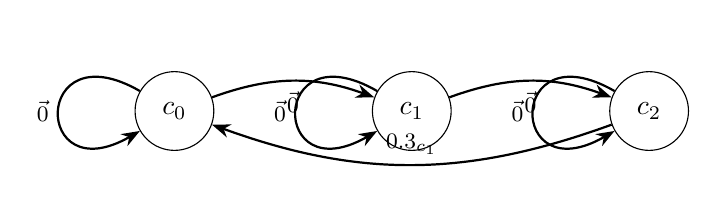
\begin{tikzpicture}[
    node distance=2cm,
    compartment/.style={circle, draw, minimum size=1cm},
    arrow/.style={->, >=Stealth, thick}
]
    % Nodes
    \node[compartment] (c0) {$c_0$};
    \node[compartment, right=of c0] (c1) {$c_1$};
    \node[compartment, right=of c1] (c2) {$c_2$};
    
    % Edges
    \draw[arrow, bend left=20] (c2) to node[above] {\footnotesize $0.3_{c_1}$} (c0);
    \draw[arrow, bend left=20] (c0) to node[below] {\footnotesize $\vec{0}$} (c1);
    \draw[arrow, bend left=20] (c1) to node[below] {\footnotesize $\vec{0}$} (c2);
    
    % Self-loops (optional, if needed)
    \foreach \n in {c0,c1,c2} {
        \draw[arrow] (\n) to[out=150,in=210,looseness=8] node[left] {\footnotesize $\vec{0}$} (\n);
    }
\end{tikzpicture}
\end{document}